\section{GHio-Ca}
\label{sec:ghioca}
In this section we will provide some salient features implemented by our application, mainly regarding the architectural and implementation choices that we made during development.

\subsection{Application description}
GHio-Ca is an Android application that gives to a user the possibility to make image recognition on her pictures. This application embed some camera features in order to make possible to take a photo and recognize it, but it also allows to pick a picture from the local storage and launch the classification process on it.
GHio-Ca is specifically designed to recognize objects and text: the only limitation is that the user has to choose it before starting the recognition process from the hamburger menu placed in the \texttt{MainActivity}.
The overall application is mainly composed by four activities.

\subsubsection{\texttt{SplashActivity}}
This view (Figure~\ref{fig:splash}) is needed in order to obtain from the user the necessary permissions (network access, camera access, access to  the storage).
\begin{figure}[h]
    \centering
    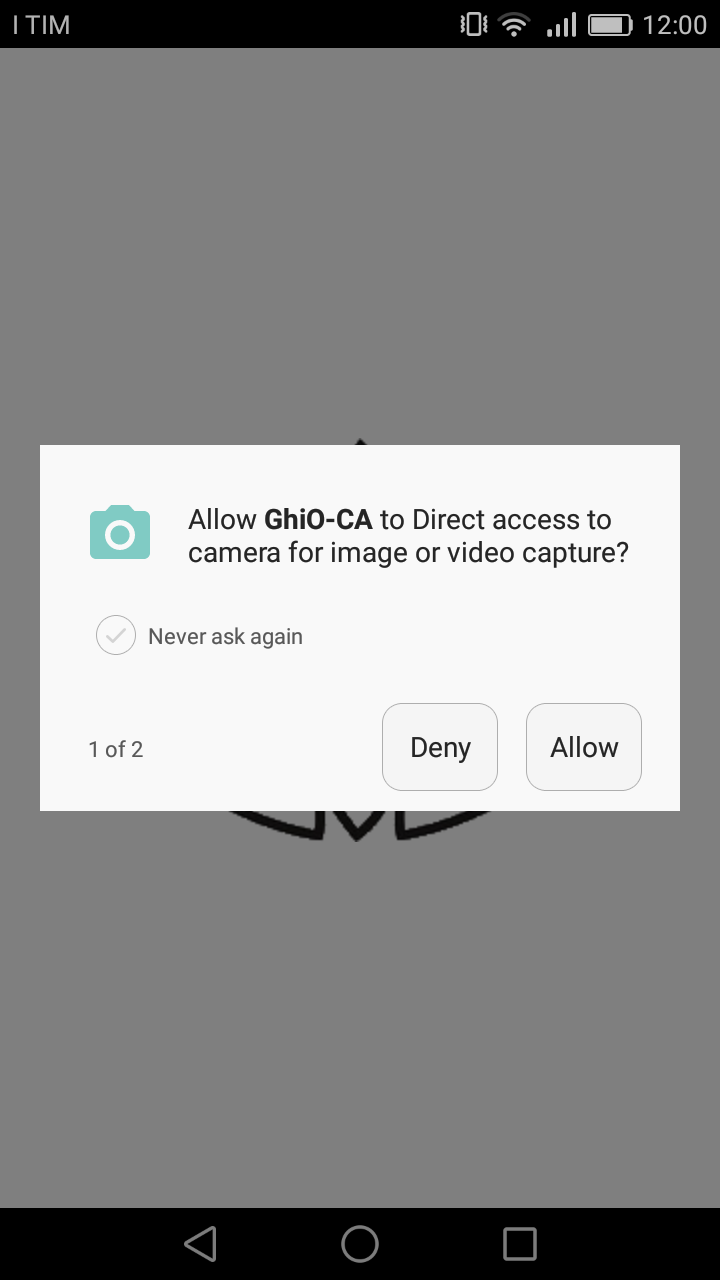
\includegraphics[width=0.2\textwidth]{../img/splash}
    \caption{Screenshot of \texttt{SplashActivity} during authorization request}
    \label{fig:splash}
\end{figure}

\subsubsection{\texttt{CameraPreviewActivity}}
This activity (Figure~\ref{fig:mainActivity}) shows to the user a camera interface, with the possibility to take photos, turn off the flash, switch to frontal camera (if present) and to access to the gallery in order to pick a file instead of taking a picture. In the top left corner is present the hamburger menu: it allows user to choose the size of picture taken, it reminds the user to turn on the Wi-Fi sensor on every access and it allows to switch from the image recognition functionality to the character optical recognition feature and vice-versa.
\begin{figure}[h]
    \centering
    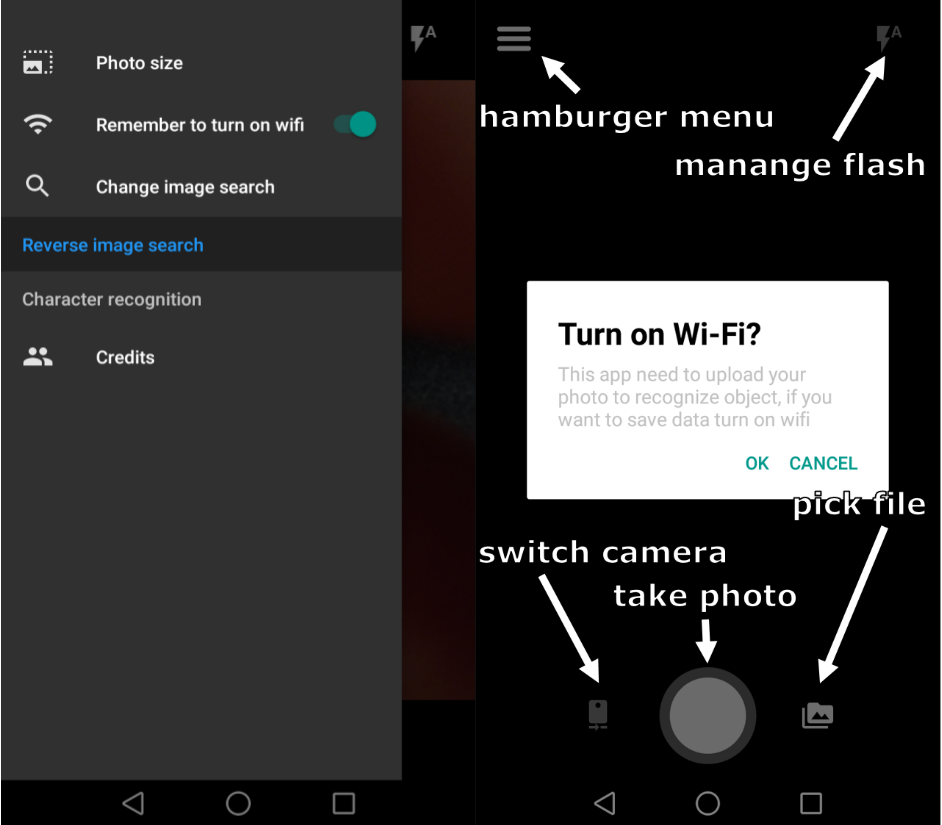
\includegraphics[width=0.30\textwidth]{../img/main_activity}
    \caption{Screenshots of \texttt{CameraPreviewActivity}, with the hamburger menu open and closed}
    \label{fig:mainActivity}
\end{figure}

\subsubsection{\texttt{ResultActivity}}
There are two different activities (Figure~\ref{fig:imageResultActivity}), depending on the type of image recognition chosen:
\begin{itemize}
	\item If the ``reverse image search'' functionality is enabled, then \texttt{ResultActivity} contains a photo thumbnail, a description and a list of tags. Any tag can be deselected by the user if it doesn't fit the image.
    \item Instead, with ``optical character recognition'' activated, \texttt{ResultActivity} displays the photographed text and its OCR translation. The user is able to pick another translation from a drop down menu.
\end{itemize}

\begin{figure}[h]
    \centering
    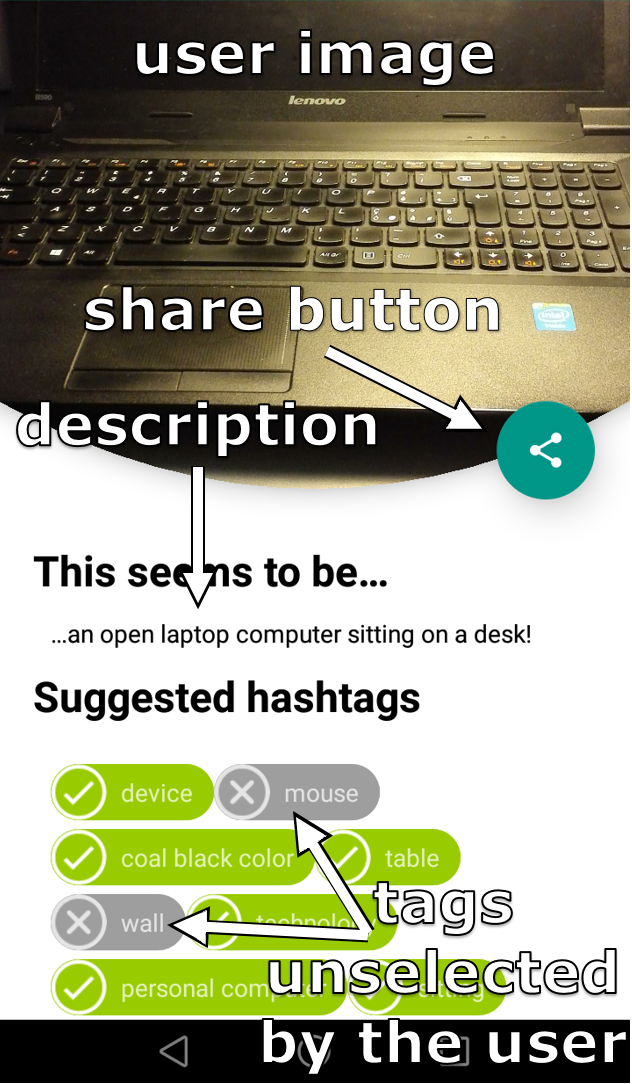
\includegraphics[width=0.18\textwidth]{../img/image_result_activity}
    \caption{Screenshots of \texttt{ResultActivity} for image recognition}
    \label{fig:imageResultActivity}
\end{figure}

\subsection{Libris}
Libris\footnote{\url{https://github.com/Augugrumi/libris}} (Library Reverse Image Search) is a library that we developed in order to 
simply the image recognition process. This library task is to make calls to the different services that we used, in order to fulfill the image or character recognition, defining an interface for the results.

All the requests return a response in \texttt{JSON} format, that will is parsed. The more informative fields are embedded in a object, different for every service, which is returned. If some error occur during the request an \texttt{IOException} will be thrown.

For image recognition Libris gives the possibility to use all the services listed in Section~\ref{sec:introduction}, except for Free OCR. In order to provide the Google Reverse Search Image service, we programmatically search on Google the image, picking up the best returned result.

For Character recognition Libris gives the chance to use: Watson OCR (still in beta), Azure OCR and OCR Space (free version).

\subsection{CameraFragment}
CameraFragment\footnote{\url{https://github.com/Augugrumi/CameraFragment}} is a library that simplify the camera usage in Android. It is 
open source and freely available on Github. Because of some issues in the library, mainly caused by the wrong management of Android \texttt{Camera1} and \texttt{Camera2}, and due to the fact that some parts of that library differed from the one expected in GHio-Ca, we decided to modify that project, changing the some parts.

\subsection{Architecture}
GHio-Ca is principally composed by three layers (Figure~\ref{fig:architecture}): (i) the one that manages network connectivity, uploads of photos to the server and makes requests to different services in order to make the image recognition or the translation of certain pieces of text; (ii) the camera layer, that manages the photo capturing process and storage on the devices, and (iii) the layer that
connects all the pieces together. 

These layers are maintained as loose coupled as possible, in order to make it easy to change services used without making important changes to the overall application (e.g changing the process of capturing a photo without modifing the networking layer).

\begin{figure}[h]
    \centering
    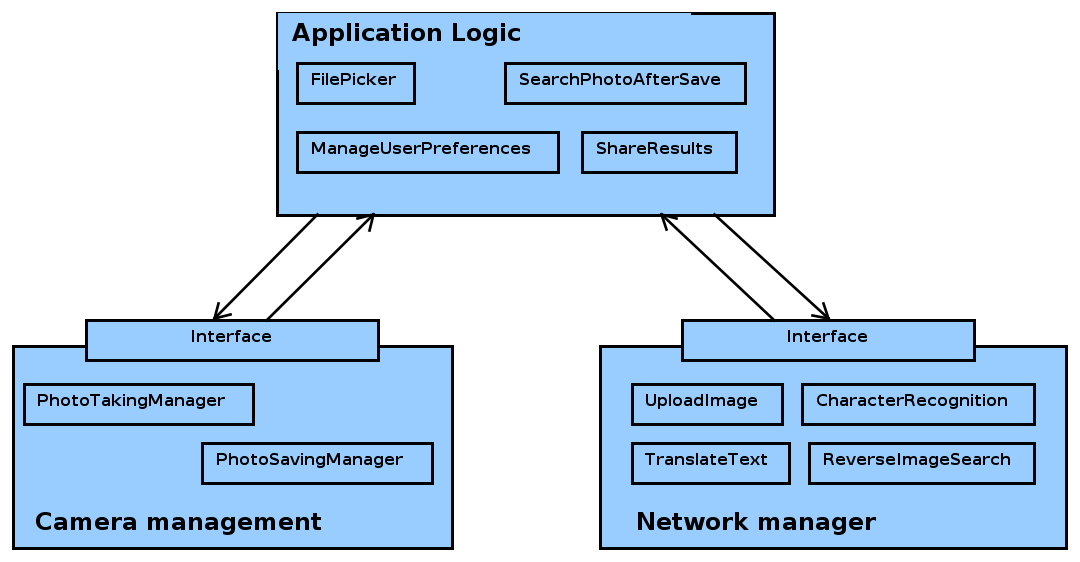
\includegraphics[width=0.50\textwidth]{../img/ghioca_macro_component}
    \caption{GHio-Ca architecture}
    \label{fig:architecture}
\end{figure}

Since we need to make network calls to recognize an image, we implemented a utility class that offers the possibility to create \texttt{AsyncTask}s, different for every service, that will be executed on a thread pool (in order to make possible to fulfill more tasks at same time). Each of those \texttt{AsyncTask}s must be associated to a listener, in order to collect all the results of the search. Practically, classes that implement the interface \texttt{Listener} expose methods \texttt{onStart()}, \texttt{onFailure()} and \texttt{onSuccess()}, that are called from the \texttt{AsyncTask}. The first one is called in \texttt{onPreExecute()} method, \texttt{onFailure()} is invoked in \texttt{onPostExecute()} if during the \texttt{doInBackground()} method some error occurred and the latter one is called if the \texttt{doInBackground()} method is executed without any issue, during \texttt{onPostExecute()}.

Thanks to the possibility of detect image recognition process failure, and since we use more services, we implemented some robustness feature in our application, enabling it to return an error to the user only if all services fail. The scenario where, even if the application could start the image recognition process but it could not be able to finish it, could still occurs (e.g. caused by a network fault).

If no errors occur, we decided to skim results based on the probability that a word (or group of words) could be correlated to the user picture. So, if the service provides this feature, we only take result that have an high probability, setting the threshold to 70\% (we fixed it empirically). If the service does not provide probability, it generally divide results in two sets based on the fact that a 
certain word could be more or less correlated to the picture. In that case we present to the user only the more related results.

This layer not only has responsibility to search the image but it ha to offer the possibility to upload the image that has to be recognized. Because of limitation of some services and to save user data, we decided to upload the photo into a server, and pass to the different services the URL of the image. With this approach, we reduce bandwidth usage: the user needs to upload the photo only once and can take advantage of the URL to make the recognition with more services.

The camera layer, instead, has only to manage the photo taking process, in order to make possible to take a photo and save it on the user smartphone. These activities are fulfilled using the Camera Fragment library. It uses a fragment in order to show to the user a preview of the photo and, when the user touch on the button for taking the photo, saves the image in a specific folder using a listener (in our case, the GHio-Ca folder, inside Android default picture folder). In order to recognize the photo taken, we have decided to create a listener that has to listen to this process and, when the image is successfully saved on the smartphone, it starts the image recognition process. 
This layer has also to give the user the ability to select the camera (frontal or back), to manage flash (turn on/off or choose automatic option) and to enable the user to choose the size of the photos.

The last layer is the one that has to connect the previous two layers. In fact, this layer has to create listeners both for the camera and the search. \todo{}It has to remember user search option choose in order to create the right kind of listener, \texttt{AsyncTask} for the search and in order to format the results that will be displayed to the user. Moreover, it manages the application sharing process: as a matter of fact, after a research, the application gives the possibility to the user to share the photo on different social networks and through e-mail. For some of them (Facebook, Twitter, Instagram, Whatsapp, Linkedin) there is a specific implementation, if the usage of a API is neededM for the others, the default Android \texttt{IntentChooser} is used. 